
\section{Appendix}

\subsection{Energy spectrum}
\label{sec:spectrum}
The discrete-time Fourier transform of the signal $x(t)$ with period $T$ is given by 
\begin{equation}
    X_j = \sum_{i=1}^{N} x(t_i) \exp\left(-\frac{2\pi}{T} ji t_i\right), 
\end{equation}
where $t_i = \frac{iT}{N}$. $\frac{j}{T}$ is the frequency. $j$ is called the frequency mode. Let $\Delta = \frac{1}{N}$ be the time step. The spectrum is defined as the product of the Fourier transform of $x$ with its conjugate:
\begin{equation}
    S_{j} = \frac{2\Delta^2}{T} X_j X_j^{*},
\end{equation}
where $X_j^{*}$ is the complex conjugate. In practice, the statistics are computed over all pixel locations and channels of randomly generated trajectories. $T=1$ and the sampling frequency is 1000 Hz to avoid aliasing. Figure~\ref{fig:spectrum} visualizes the energy spectrum of ODE trajectories sampled from the diffusion model "DDPM++ cont. (VP)" trained by \cite{song2020score} on CIFAR10. We observe that most power concentrates in the regime where the frequency mode is less than 5. 

\begin{figure}[htbp]
    \centering
    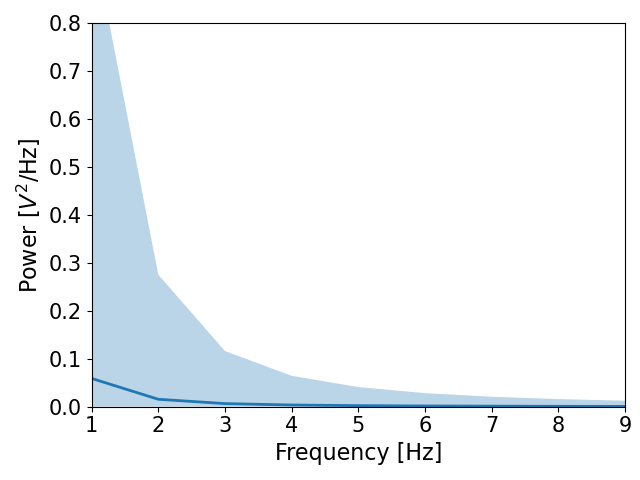
\includegraphics[width=0.5\columnwidth]{figs/power_spectrum.png}
    \caption{Power spectrum of the ODE trajectories sampled from "DDPM++ cont. (VP)" model trained by \cite{song2020score} on CIFAR10. The mean is computed over all pixel locations and channels of randomly generated trajectories. Most power concentrates in the $\leq 5$ Hz regime. The shaded region represents the maximum and minimum power.  }
    \label{fig:spectrum}
    % \caption{Compact spectrum and DFNO architecture design.}
\end{figure}

\subsection{Background: neural operators}
\label{sec:neural_operator}
Let $\mathcal{A}$ and $\mathcal{U}$ be two Banach spaces and $G: \mathcal{A} \rightarrow \mathcal{U}$ be a non-linear map. 
Suppose we have a finite collection of data $\{a_i, u_i\}_{i=1}^{N}$ where $a_i\sim \mu$ are i.i.d. samples from the distribution $\mu$ supported on $\mathcal{A}$ and $u_i=G(a_i)$.
Neural operators aim to learn $G_{\phi}$ parameterized by $\phi$ to approximate $G$ from the observed data by minimizing the empirical risk given by
\begin{equation}
    \min_{\phi} \mathbb{E}_{a\sim \mu} \|G(a) - G_{\phi}(a)\|_{\mathcal{U}} \approx \min_{\phi} \frac{1}{N} \sum_{i=1}^{N} \|u_i - G_{\phi}(a_i)\|_\mathcal{U}.
\end{equation}


The architecture of neural operators is constructed as a stack of kernel integration layers where the kernel function is parameterized by learnable weights. This architecture utilizes the convolution theorem on abelian groups. Among different neural operator architectures, Fourier neural operator~\cite{li2020fourier} stands out and is one of the most efficient machine learning methods for scientific computing problems involving PDE
\cite{yang2021seismic,wen2022accelerating}. It is shown to possess the crucial discretization invariance and universal approximation properties of universal operators~\citep{kovachki2021universal,kovachki2021neural}.


\subsection{Extended set of generated samples}
We provide an extended set of randomly generated samples from our ImageNet-64 model in Figure~\ref{fig:images_set1}. 
\begin{figure}[htbp]
    \centering
    \includegraphics[width=0.6\textwidth]{figs/dsno-set1-min.pdf}
    \caption{Random samples generated from DSNO on ImageNet-64.}
    \label{fig:images_set1}
\end{figure}




\subsection{Generalization to different resolution}

Figure~\ref{app_fig:demo_imagenet} visualizes the predicted trajectory of DSNO in temporal resolution 8 on ImageNet-64 while it is trained on temporal resolution 4. Although the resulting trajectories do not look perfectly smooth, it still demonstrates the generalization ability of DSNO to unseen time resolutions.



% \subsection{Related work}
% \paragraph{ODE-based sampling.}
% ODE-based samplers are much more widely used in practice \cite{stablediffusion} than SDE-based methods because they can take large time steps by leveraging some useful structures of the underlying ODE such as semi-linear structure and the form of exponentially weighted integral \cite{lu2022dpm, zhang2022fast}. Existing works \cite{song2021denoising, bao2021analytic, zhang2022fast,dockhorn2022genie} have greatly reduced the number of discretization steps to 10-50 in time while keeping the approximation error small to generate high-quality samples. The exponentially weighted integral structure of the solution trajectory revealed by prior works also inspired our design of the temporal convolution block. We note that these advanced numerical solvers allow us to approximate the solution operator with less computation cost, which greatly speeds up our training data generation process and also benefits other training-based methods.  
%  % In this paper, we also use some of the advanced ODE-based solvers to generate our training set for DSNO. 

% \paragraph{Operator learning for solving PDEs.}
% Neural operators are deep learning models that are designed for mappings between function spaces, i.e., continuous functions~\cite{li2020neural,kovachki2021universal}. They are widely deployed as the de facto deep learning models in scientific computing when dealing with partial differential equations (PDE).
% % Operator learning is a successful learning paradigm in the scientific computing area for solving partial differential equations. It contains a diverse class of methods including DeepOnet-based methods and neural operator methods including \citet{li2020neural, li2020multipole, li2020fourier}. 
% Among these methods, Fourier neural operator stands out and is one of the most efficient machine learning methods for scientific computing problems involving PDE
% \cite{yang2021seismic,wen2022accelerating}. 
% This architecture utilizes the convolution theorem on abelian groups and is shown to possess the crucial discretization invariance and universal approximation properties of universal operators~\citep{kovachki2021universal,kovachki2021neural}, which motivates our design of the temporal convolution block in our method.

% \paragraph{Training-based sampling.} Training-based methods typically train a neural network surrogate to replace some parts of the numerical solver or even the whole solver. This category includes various methods from diverse perspectives such as knowledge distillation \cite{luhman2021knowledge, salimans2021progressive}, learning the noise schedule \cite{lam2021bilateral, watson2021learning}, learning the reverse covariance \cite{bao2022estimating}, which require extra training. Training-based methods usually work in the few-step regime with less than 10 steps. Direct \citet{luhman2021knowledge} is the first work to get descent sample quality on CIFAR10 with one model evaluation but it suffers from overfitting and its sampling quality drops dramatically compared to the original numerical sampling methods in diffusion models. The current SOTA progressive distillation \cite{salimans2021progressive} reduces the number of steps down to 4-8 without losing much sample quality. However, it has the same issue as knowledge distillation in the limit of one function evaluation. Some other methods~\cite{xiao2021tackling,vahdat2021score} combine diffusion models with other generative models such as GAN and VAE to enable fast sampling. 

% \paragraph{Diffusion + GANs.} 

\subsection{Further discussion}
\paragraph{Future work}
There are several directions we leave as future work. First, guided sampling of diffusion models is widely used in various applications but accelerating guided sampling is also more challenging~\cite{meng2022distillation}. How to adapt DSNO for sampling Guided diffusion model will be an interesting next step. 
Second, the temporally continuous output of DSNO provides another level of flexibility compared to distillation-based methods and is readily available for applications such as DiffPure~\cite{nie2022DiffPure} that require fast forward/backward sampling from diffusion models at various temporal locations. DSNO could potentially reduce the inference time in those applications.
We leave the exploration of those applications to future work. Last but not least, transformer-based architectures have shown their promising capacity for diffusion models~\cite{peebles2022scalable, bao2023all} in high-resolution image generation. It is natural to integrate our temporal convolution layers into these diffusion transformers as the temporal blocks operate solely on the temporal dimension regardless of how the pixel space is modeled. The resulting new architecture could also potentially serve as a new architecture design for other problems where the dynamics are continuous in time. 

\paragraph{Reducing data collection cost with advanced solvers.} While we primarily use DDIM solver to collect data for fair comparison in this paper, it is worth noting that advanced numerical solvers like DPM solver\cite{lu2022dpm} can approximate the solution operator with less computation cost, which will greatly speed up our training data generation process. Our final implementation includes examples of using DPM solvers in our GitHub repository \href{https://github.com/devzhk/DSNO-pytorch}{https://github.com/devzhk/DSNO-pytorch}. 



\begin{figure*}[ht]
        \centering
        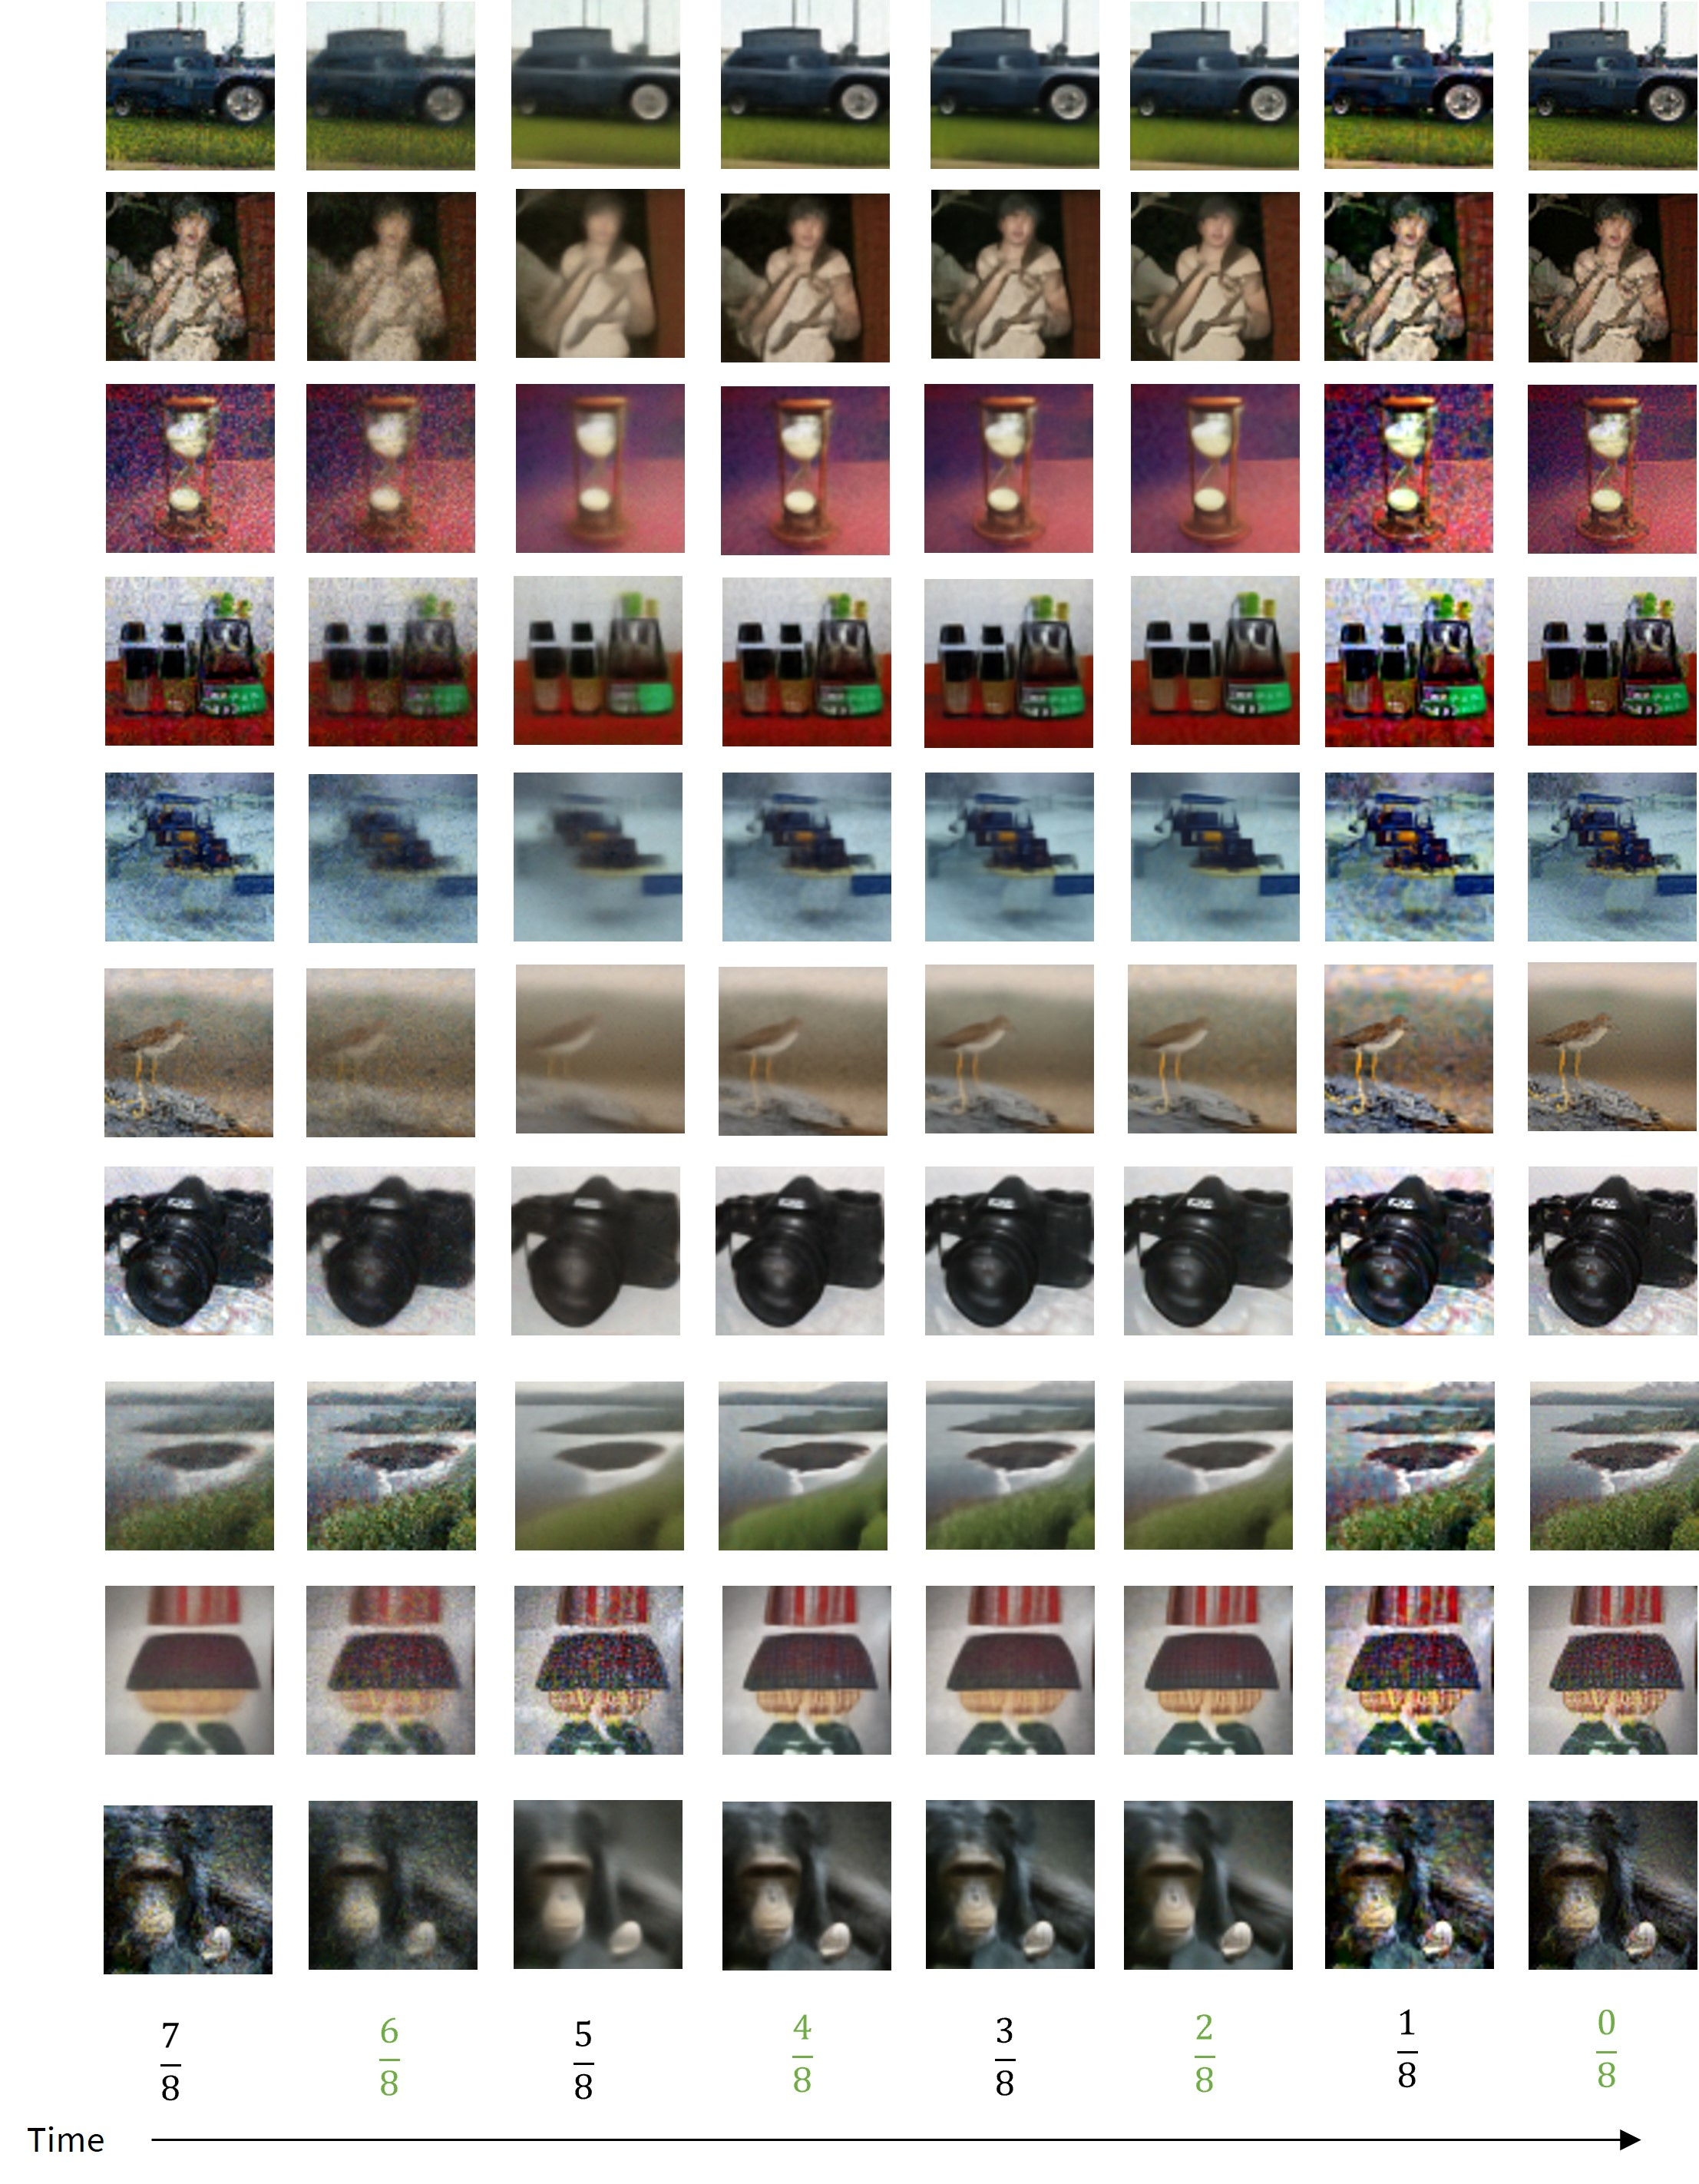
\includegraphics[width=0.75\textwidth]{figs/demo_high-res-app-1.jpg}
        \caption{The predicted trajectory of DSNO with a temporal resolution of 8 on ImageNet-64. We train the DSNO with a temporal resolution of 4 and then use it to predict the trajectory with a temporal resolution of 8. Time locations marked green are the points that DSNO is trained with. Black time locations are the points that DSNO never saw in the training set. }
        \label{app_fig:demo_imagenet}
\end{figure*}